	%====================================================================================================
	% ?????
	%====================================================================================================
	% TCC
	%----------------------------------------------------------------------------------------------------
	% Autor				: Jasane Schio
	% Orientador		: Gedson Faria
	% Co-Orientador		: Angelo Darcy
	% Instituição 		: UFMS - Universidade Federal do Mato Grosso do Sul
	% Departamento		: CPCX - Sistema de Informação
	%----------------------------------------------------------------------------------------------------
	% Data de criação	: 01 de Outubro de 2015
	%====================================================================================================
	
	\definecolor{dkgreen}{rgb}{0,0.6,0}
	\definecolor{gray}{rgb}{0.5,0.5,0.5}
	\definecolor{mauve}{rgb}{0.58,0,0.82}
	
	\lstset{frame=tb,
		language=C++,
		aboveskip=3mm,
		belowskip=3mm,
		showstringspaces=false,
		columns=flexible,
		basicstyle={\small\ttfamily},
		numbers=none,
		numberstyle=\tiny\color{gray},
		keywordstyle=\color{blue},
		commentstyle=\color{dkgreen},
		stringstyle=\color{mauve},
		breaklines=true,
		breakatwhitespace=true,
		tabsize=3
	}
	\chapter{Metodologia e Desenvolvimento} \label{Cap:Processamento}
	
			Para o desenvolvimento foi escolhida a biblioteca OpenCV por ser OpenSource, multiplataforma, uma grande quantidade de métodos e algoritmos já implementados	e pelo seu rápido desempenho de máquina.
			A linguagem escolhida para o desenvolvimento foi o C++ pois é uma linguagem de programação compilada, o que torna sua execução mais rápida que as linguagem interpretadas, tendo assim grande desempenho e por ser uma linguagem orientada objeto. 
			
			O sistema desenvolvido é separado em duas partes: Processamento e Interface Gráfica.
			A parte de Processamento é onde são feitas as partes de aquisição de imagem, processamento de imagem, conversão de imagem para modelo de cor HSV, seleção de pontos de cor e contagem de ocorrência de cor. Já a interface gráfica, é a onde ocorre a entrada do usuário para assim ser feita a calibração manual de mínimos e máximos de cada cor.
		
	
	Passos do projeto:
	\begin{description}
		\item[Aquisição de imagens em vídeo:] Nesse passo as imagem são adquiridas via câmera USB.
		
		\item[Identificação de Objetos:]
				 Durante o processo de aquisição de imagem são selecionados os objetos, quais serão usados como base para a detecção de máximos e mínimos de cores.
		\item [Cálculo de Mínimos e Máximos:]
		 Nessa etapa são levados em consideração os objetos teste. A imagem é "varrida"  por pixel na localidade dos objetos-teste e assim são salvos seus valores e feito a contagem de ocorrências de cada cor.		
	\end{description}


	\section{Projeto}
	\subsection{Organização do Projeto}
	 O projeto foi desenvolvido seguindo o paradigma de programação conhecido como  Orientação à Objetos, esse paradigma baseia-se na utilizaç~ao de objetos individuais para criaçao de um sistema maior e complexo. A IDE usada para o desenvolvimento foi a QT Creator. Esta separada o projeto em três pastas, Headers, Sources e Forms. Na pasta Headers estão os arquivos de cabeçalho(.h) onde estão as declarações dos métodos e variáveis usados nas classes  executáveis. Já na pasta Sources estão os arquivos fonte(.cpp), são nesses arquivos que os métodos declarados nos arquivos da pasta Header são implementados. Na pasta Forms está o arquivo de interface gráfica(.ui) que é usado no projeto para ser a ponte entre o usuario e as funções do sistema.
	 
	\begin{figure}[!h]
		\centering
		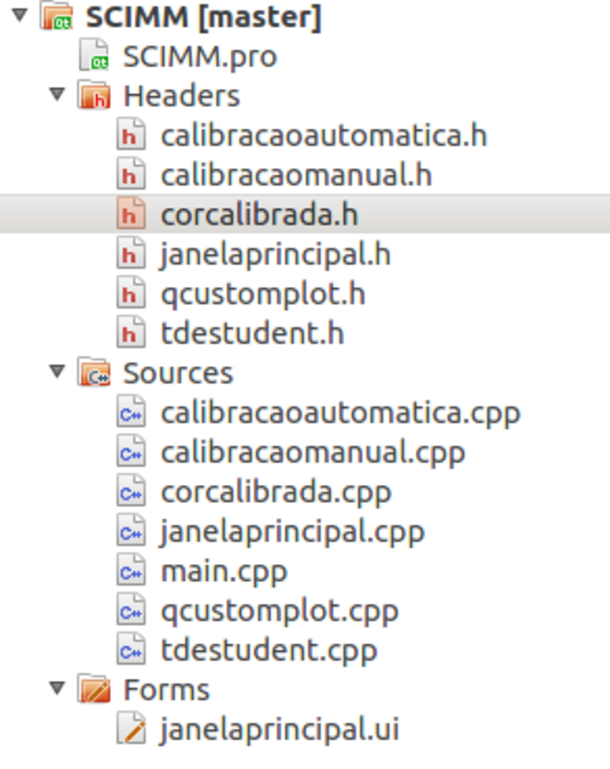
\includegraphics[width=0.2\textwidth]{organizacaoProjeto.pdf}
		\caption{Organização das pastas do projeto}
		\label{Organizacao do Projeto}
	\end{figure}
	Cada arquivo de cabeçalho possui um arquivo fonte correspondente, formando assim uma Classe, com exceção do arquivo fonte main, pois para este arquivo não há a necessidade.
	As classes desenvolvidas no projeto são:
 calibracao, manual, automatica, corcalibrada, janelaprincipal e tdestudent. Já a classe qcustomplot é um componente para auxilio em plotagem de gráficos e vizualização de dados\cite{QCustomPlot}.
Para melhor entendimento da interação entre as classes a figura 3.2 trás o diagrama de classes do projeto.
	 \begin{figure}[!h]
	 	\centering
	 	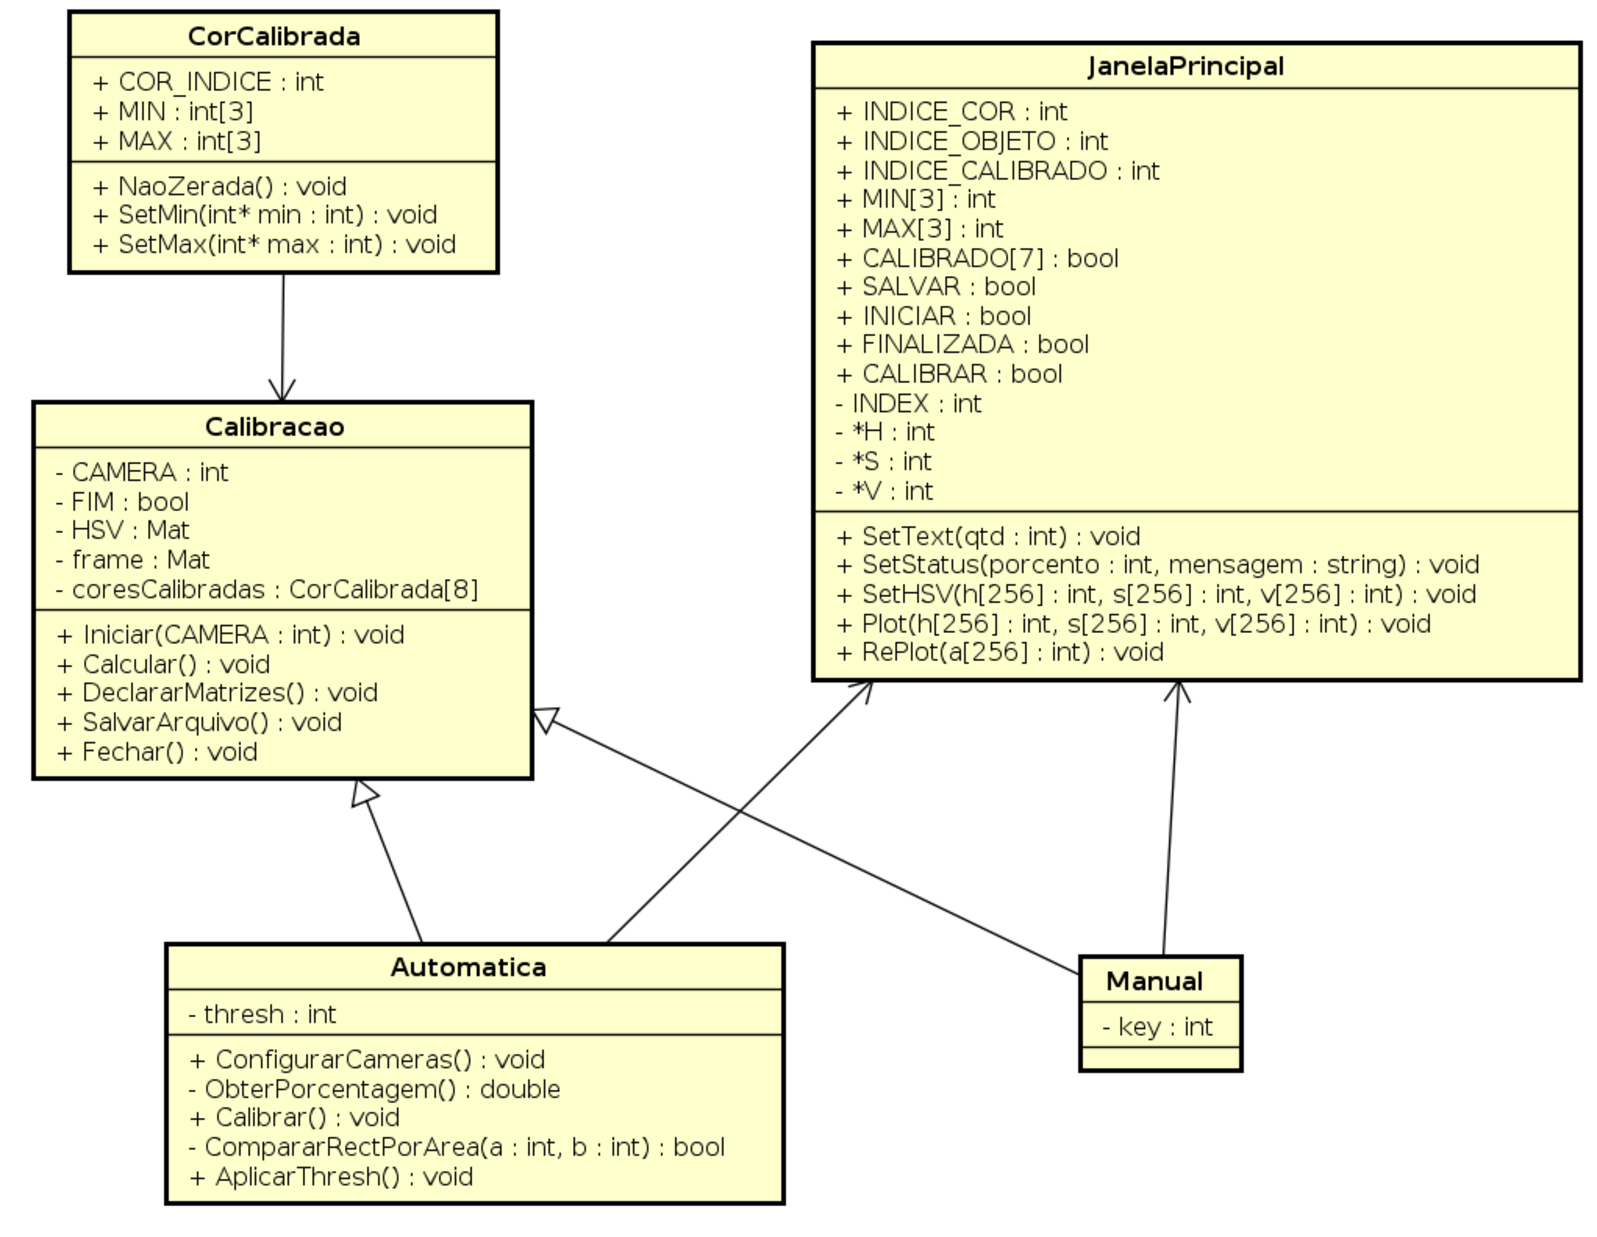
\includegraphics[width=0.8\textwidth]{diagramadeclasse.pdf}
	 	\caption{Diagrama de Classes do projeto}
	 	\label{DiagramaDeClasse}
	 \end{figure}\newpage


\subsection{Classes}
	\begin{description}

	\item [main] esta é a classe executavel do sistema, ela inicia o programa e em seguida chama a classe de interação grafica \textbf{janelaprincipal}  
	
	\item [janelaprincipal]	classe que faz a interação com o usuario e que de acorco com esta interação seleciona o tipo de calibração, e seus parametros, para então ser feita a analize dos pixeis	
		
	\item [calibracao] classe "pai" que contem os metodos e variaveis que virão a ser usadas por ambas as classes \textbf{manual} e \textbf{automatica}
	
	\item [manual] classe que contem os metodos, calculos e variaveis necessarias para a calibração manual
	
	\item [automatica] classe que contem os metodos, calculos e variaveis necessarias para a calibração automatica
			
	\item [corcalibrada] classe que salva o indice da cor já calibrada e seu intervalo de valores
	
	\item [tdestudent] esta é a classe que faz o calculo probabilistico conhecido com TdeStudent
	

	\end{description}

	

	\section{Fluxo do Sistema}
O sistema possui um fluxo principal e dois subfluxos de acordo com o tipo de calibração escolhida. A Figura 3.3 mostra o fluxo principal do sistema.
		\begin{figure}[!h]
			\centering
			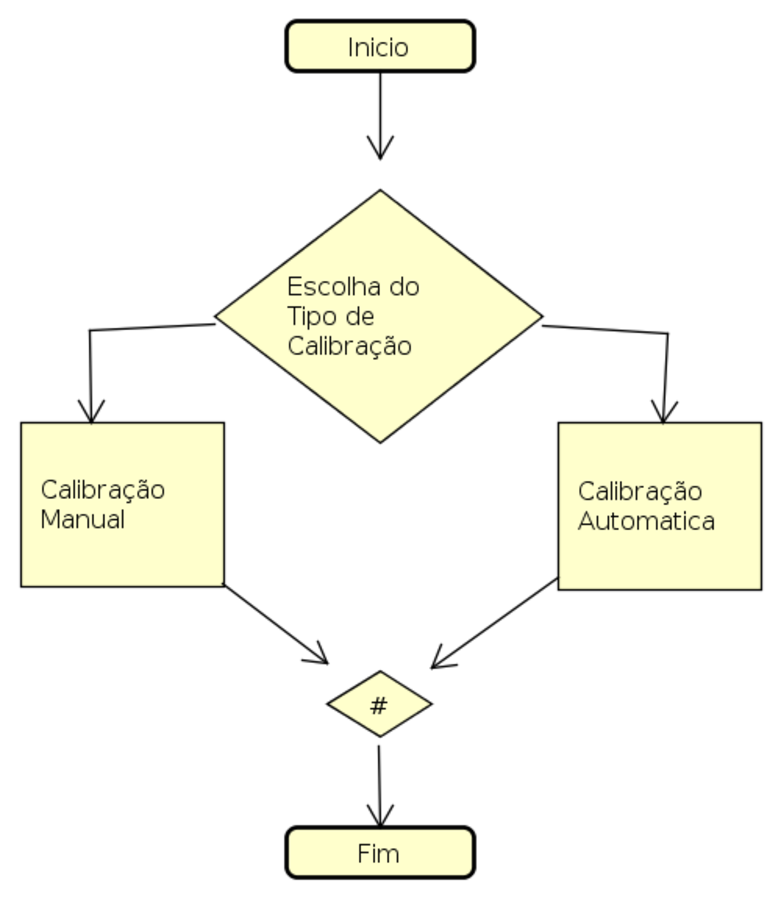
\includegraphics[width=0.45\textwidth]{fluxoprincipal.pdf}
			\caption{Diagrama de Fluxo}
			\label{FlowCHart}
		\end{figure}
		
	\subsection{Fluxo de Calibração Manual}	
	Nesta etapa são declaradas todas as variáveis necessárias para execução do sistema, tanto da interface gráfica quanto da parte de processamento da imagem. Também é nesta etapa que se verifica a câmera esta disponível ou não. Caso a câmera não esteja disponível o sistema não é inicializado.
	
		\begin{figure}[!h]
				\centering
				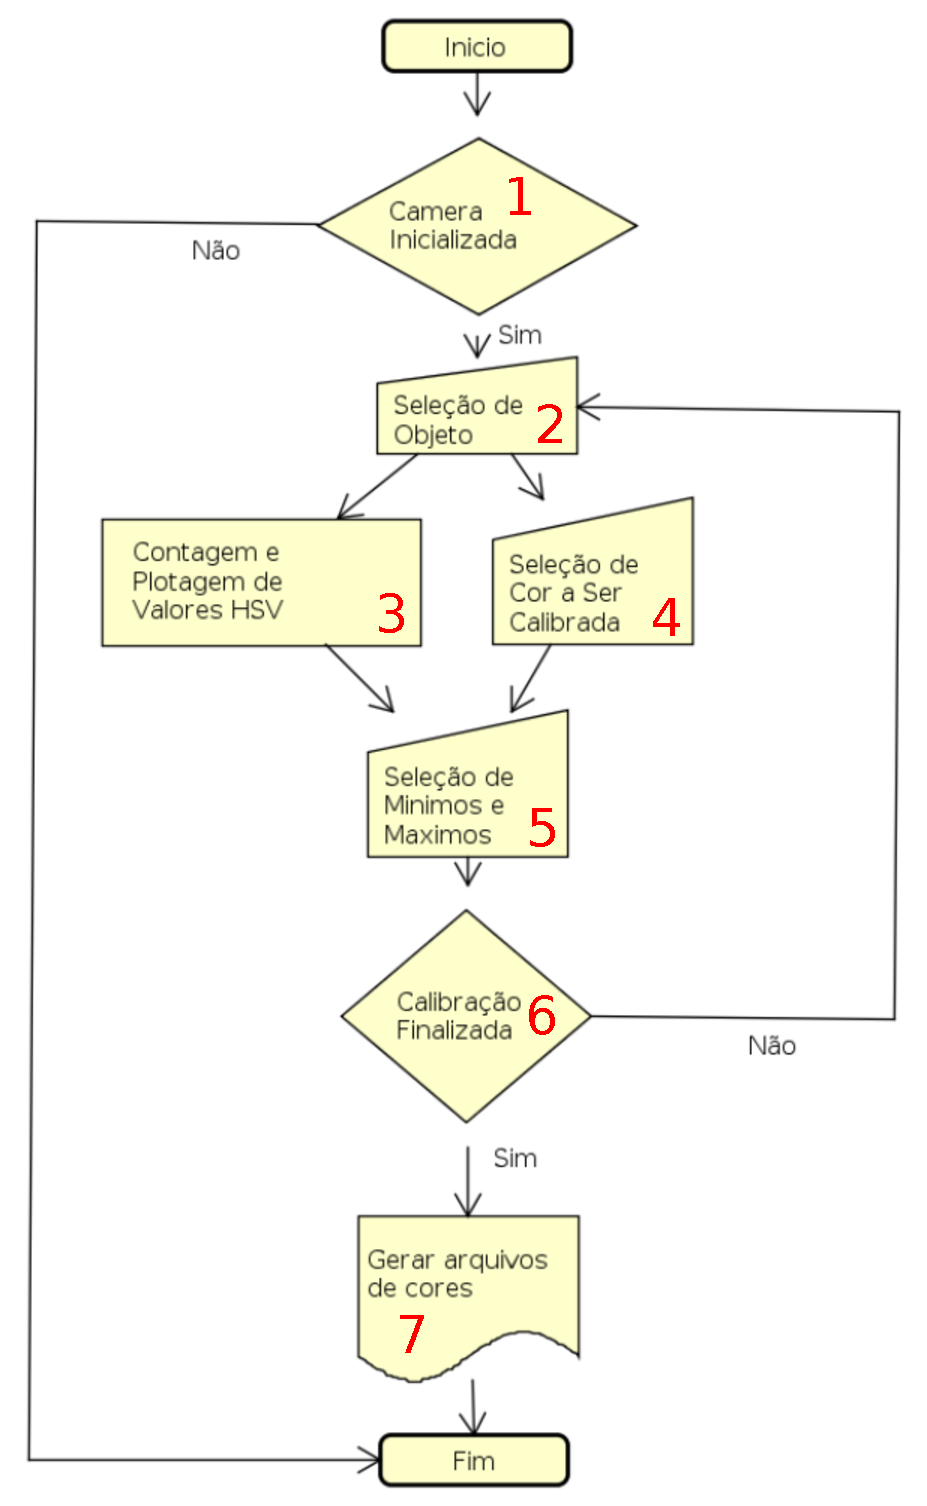
\includegraphics[width=0.45\textwidth]{fluxomanual.pdf}
				\caption{Diagrama de Fluxo Manual}
				\label{DiagramaDeFluxoManual}
			\end{figure}
	\subsection{Fluxo de Calibração Automatica}		
		Após ter sido inicializado com sucesso o programa dispõe sua interface gráfica que é separada entre 2 janelas, a Janela 1, Gráfico, e a Janela 2, Seleção de Cores, detalhadas no Capítulo 4, sendo então possível iniciar o processo de calibração. 
